\section{Grundlagen}
%Im Grundlagenkapitel stellen Sie das Basiswissen für die weiteren Kapitel vor. 
%Hierzu können neben theoretischen Konzepten auch die historische Entwicklung 
%und aktuelle Forschungsvorhaben gehören. Idealerweise bedient man sich hier 
%mehrerer verschiedener Quellen, um die Ausführungen zu belegen.

%Nachfolgend werden einige Formalitäten der Arbeit dargestellt.






In dieser Arbeit soll ein Vorgehensmodell für bestehende 
Client-Server-Anwendungen in die Cloud zu 
Salesforce entwickelt werden. Basis für diese Entwicklung ist das 
Fünf-Phasen-Modell aus \citeflow{fivephases} und 
\citeflow{exploring_the_factors}. Bevor dieses Modell vorgestellt 
wird, soll zunächst der Begriff "`Cloud"' definiert und die Charakteristika 
der Cloud vorgestellt werden. Um die Chancen und Risiken einer Migration 
realistisch abschätzen 
zu können, ist es zudem nötig, die Faktoren zu kennen, die den Erfolg einer 
Migration bestimmen. 
\subsection{Cloud-Computing}
Da die Definition von "`Cloud-Computing"' des National Institute of Standards 
and Technology (NIST) \pcite{}{}{NIST} in \citeflow{thoughtsOnCloud} als gute 
Grundlage geschätzt wird und auch in \citeflow{fivephases}, in dem das 
Fünf-Phasen-Modell vorgestellt wird, als Basis dient, übernehme ich die
Definition in übersetzter Form aus \citeflow{softwareindustrie2015}:
\begin{cloudcomputing}
"`Ein Modell, das einen komfortablen, bedarfsabhängigen und netzbasierten 
Zugriff auf eine gemeinsam benutzte Menge konfigurierbarer Rechenressourcen 
ermöglicht, die schnell, mit geringem Verwaltungsaufwand und ohne (menschliche) 
Interaktion mit einem Anbieter bereitgestellt und wieder freigegeben werden 
können."'
\end{cloudcomputing}
Laut NIST besteht die "`Cloud"' als Modell neben fünf Charakteristika und drei 
Service Modellen aus vier Einsatzmodellen (im Englischen: "`Deployment 
Models"'). Da sie für das Verständnis des Fünf-Phasen-Modells nebensächlich 
sind, wird hier nur kurz auf die Einsatzmodelle eingegangen. In ihnen geht es 
darum, ob die Cloud ausschließlich von einer Organisation, von einer bestimmten 
Gruppe von Organisationen oder von der Öffentlichkeit genutzt wird, wobei auch 
Mischformen als Möglichkeit genannt werden. \pcite{}{}{NIST}

\subsubsection{Charakteristika}
Die fünf Charakteristika von Cloud-Computing, die in \citeflow{NIST} genannt 
werden, lauten zusammengefasst:

\begin{description}
	\item[Selbstbedienung bei Bedarf:] Ein Nutzer kann ohne 
zwischenmenschliche Interaktion mit dem Dienstleister die automatische 
Zuteilung von Rechenkapazitäten anstoßen.
	\item[Umfassender Zugriff über das Netzwerk:] Die Dienstleistung ist 
über das Netzwerk mit verschiedensten Geräten auf standardisierte Art und Weise 
abrufbar, zum Beispiel mit einem Internet Browser.
	\item[Geteilte Ressourcen] Kunden eines Cloud-Anbieters teilen 
sich physische oder virtuelle Rechenleistung, die dynamisch und bedarfsgerecht 
zugeteilt wird. Im Allgemeinen hat der Nutzer weder Kenntnis noch 
Kontrolle über den Ort der Speicherung und Verarbeitung seiner Daten. Abhängig 
vom Anbieter lassen sich Orte aber vertraglich festlegen. 
	\item[Schnelle Anpassungsfähigkeit] Rechenkapazitäten können dem Bedarf 
entsprechend, teilweise automatisch, schnell zugewiesen und entzogen werden. 
Auf den Kunden wirkt die abrufbare Rechenleistung oftmals unbegrenzt.
	\item[Vermessene Dienstleistung] Cloud Systeme messen und optimieren 
Ressourcennutzung automatisch und stellen die Auslastung und die Nutzung sowohl 
dem Cloud Anbieter als auch dem Nutzer zur Verfügung, da sie 
Berechnungsgrundlage für die Kosten sind.
\end{description}

\subsubsection{Service Modelle - XaaS}
Service Modelle beschreiben, welche Leistungen "`as a Service"' angeboten 
werden. Es gibt recht viele dieser Modelle - \citeflow{xAsAService} zählt 35 
Varianten - die mehr oder weniger verbreitet sind und mit "`Everything as a 
Service (XaaS)"' zusammengefasst werden. \pcite{}{95}{benlian_saas_2010} Nicht 
zwangsläufig beschränkt er sich auf Technologien, die als Dienstleistung 
angeboten werden. \pcite{}{872}{decision-making_in_cloud_computing_environments} 
\\
\citeflow{NIST} sieht drei Service Modelle vor, die sich im Anteil der 
selbst zu verwaltenden, technologischen Anteile (Integrationstiefe) 
unterscheiden und in dieser 
Hinsicht in Abbildung ~\ref{xaas_im_vergleich} mit der herkömmlichen IT 
verglichen werden. Die Wahl des Modells wirkt sich auf den 
Migrationsprozess aus. \pcite{}{213}{Pahl2013}
\begin{figure}[hb]
\begin{center}
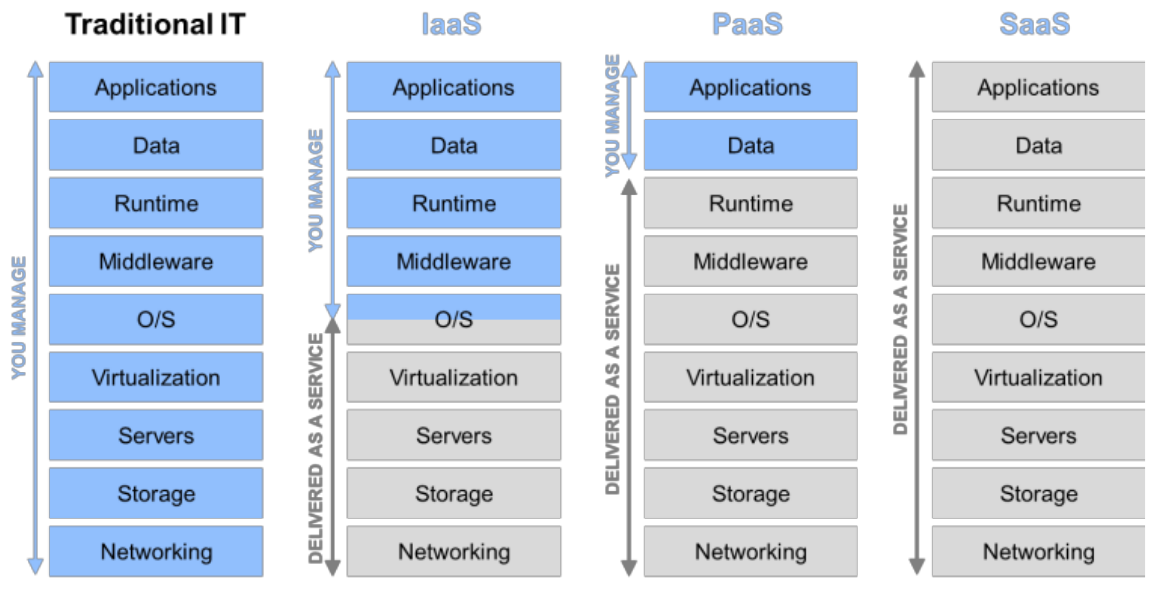
\includegraphics[width=\textwidth]{images/XaaS_im_Vergleich.png}
\caption{XaaS im Vergleich: Umfang von 
Dienstleistung und Eigenverantwortung. Aus 
\protect\citeflow{economics_of_the_cloud} }
\label{xaas_im_vergleich}
\end{center}
\end{figure}
\begin{description}
	\item[Infrastructure as a Service (IaaS)] Dem Kunden werden Netzwerk, 
Speicher und Rechenleistung zur Verfügung gestellt. Über die darauf laufende 
Software, teilweise sogar über das Betriebssystem kann selbst verfügt werden. \\
Kunden versprechen sich von IaaS vor allem Flexibilität in der Bereitstellung 
und dem Betrieb von Servern, Datenspeichern und Netzwerkressourcen. 
\pcite{}{213}{Pahl2013}
	\item[Platform as a Service (PaaS)] Der Kunde kann bereitgestellte 
oder selbst entwickelte Software in der Cloud laufen lassen und eventuell 
Einfluss auf die Anwendungsumgebung nehmen. \\
	\item[Software as a Service (SaaS)] Der Kunde kann eine vom Anbieter 
bereitgestellte Software nutzen und in begrenztem Maße konfigurieren.
\end{description}

\subsection{Die Migration bestimmende Faktoren}
\label{cha:migration_bestimmende_faktoren}
\citeflow{fivephases} identifizieren wirtschaftliche und technische Faktoren, 
die sowohl die Migrationseignung einer Anwendung als auch die Migration selbst 
beeinflussen. \\
\citeflow{decision-making_in_cloud_computing_environments} sehen viele 
Parallelen zwischen dem Outsourcen von IT zu externen 
Dienstleistern und dem Betrieb in der Cloud, weshalb sich Erfahrungen bei 
Outsourcing-Projekten bei Cloud-Migrationen 
anwenden lassen. Aus diesem Grund sind die folgenden Faktoren auch aus der
Literatur über IT-Outsourcing zusammengetragen.
\subsubsection{Wirtschaftliche Faktoren}
\begin{description}
	\item[Bereits getätigte IT-Investitionen:]
	In der Regel wachsen die bereits getätigten IT-Ausgaben mit dem 
Unternehmen und mit ihnen die Komplexität der Migration. Deshalb ist es in 
kleinen Unternehmen eher möglich, direkt zu migrieren, während bei 
größeren Unternehmen der Übergang in die Cloud wesentlich mehr Planung und 
gegebenenfalls einen parallelen Betrieb erforderlich macht.

	\item[Kosten:] In der herkömmlichen IT bestehen Kosten aus der 
"`kapitalintensiven Beschaffung der Hard- und Software sowie der Vorhaltung 
eigener Personalressourcen"' \pcite{}{}{Repschlaeger2010}. Diese Kosten sind 
zwar hoch, aber aufgrund der langjährigen Erfahrung auch vorhersagbar und in 
Budgets eingeplant. Die Migration in die Cloud dagegen bedeutet den Umstieg zu 
einem "`pay per use"'-Modell \pcite{}{}{elements_of_cloud_adoption}, von einem 
von Fixkosten dominierten Modell zu einem, das von variablen Kosten bestimmt 
ist. 
Um zu verhindern, dass Kosteneinsparungen aufgezehrt werden, ist es nötig 
den Umfang der Anwendungsnutzung und die Migrationskosten abzuschätzen.


	\item[Datensicherheit:] Bevor eine Anwendung in die Cloud migriert 
wird, sollte bedacht werden, wie kritisch die zugehörigen Daten für den 
Unternehmenserfolg sind. 
	\item[Rechtliche Restriktionen:] Vor der Migration sollte geprüft 
werden, ob rechtliche Bestimmungen auch bei einem Betrieb in der Cloud 
eingehalten werden können. 
	\item[Zuteilung von Rechenleistungen:] Anwendungen, die kurzzeitig 
große Rechenleistungen benötigen und gut skalierbar sein sollen, lassen sich in 
der Cloud wahrscheinlich kostengünstiger betreiben als auf eigenen Servern, die 
ganzjährig reserviert sind und die meiste Zeit im Leerlauf verbringen. 
\end{description}


\subsubsection{Technische Faktoren}
\begin{description}
	\item[Bestehende Infrastruktur:] Bereits die Migration einer 
einzigen Anwendung kann Änderungen in der internen IT-Infrastruktur 
erforderlich machen. Zum Beispiel wenn Daten zwischen verschiedenen Diensten 
ausgetauscht werden soll. Auch die Arbeit des Supports könnte dur
	
	\item[Sicherheitsarchitektur:] Um die Daten im Cloud-Umfeld zu 
schützen, muss das bestehende Sicherheitskonzept an die Gegebenheiten der Cloud 
angepasst werden.

	\item[Komplexität:]
	Während einfache, standardisierte Anwendungen womöglich bereits in der 
Cloud angeboten werden, steigt mit der Komplexität auch der Planungs-, 
Implementierungs und Testbedarf bei der Migration.
	
	\item[Netzwerk und Support:] Je mehr Daten in der Cloud liegen, desto 
höher ist die Abhängigkeit von einer funktionierenden Internetverbindung. Hier 
können zusätzliche Kosten für redundante Verbindungen, Verbindungen mit höheren 
Kapazitäten oder Verträge mit garantierten Reaktionszeiten im Störungsfall 
anfallen. 

	\item[IT-Fähigkeiten:] Auch wenn im Cloudbetrieb auf existierende 
Technologien und idealerweise existierende Software zurückgegriffen wird, 
erfordert die Migration dem IT-Team Fähigkeiten und Kenntnisse in den Bereichen 
Architekturen, Implementierung, Entwicklung und Betrieb ab. Hinzu kommt, dass 
der Umfang, in dem Kontrolle über die Systeme im Cloudbetrieb abgegeben wird, 
von den verantwortlichen IT-Mitarbeitern eine "`kulturelle"' Herausforderung 
darstellen kann.
	
	\item[Service Level Agreements (SLAs):] Geprüft werden sollte auch, ob 
Cloud-Anbieter SLAs bieten können, die zum unternehmerischen Bedarf 
hinsichtlich Verfügbarkeit, Vertraulichkeit und Integrität passen. Auch sollte 
geregelt sein, welche Verantwortlichkeiten der Anbieter trägt und welche 
Vertragsstrafen bei Nichteinhaltung drohen.
\end{description}

\subsection{Das Fünf-Phasen-Wasserfallmodell}
Das in \citepara{fivephases} vorgeschlagene Vorgehensmodell zur Migration 
einer Anwendung in die Cloud ähnelt dem aus der 
Softwareentwicklung bekannten, iterativen Wasserfallmodell und besteht aus den 
folgenden fünf Phasen, die in Abbildung 
\ref{fuenf-phasen-wasserfall-modell}
dargestellt sind.
\begin{figure}[!h]
\begin{center}
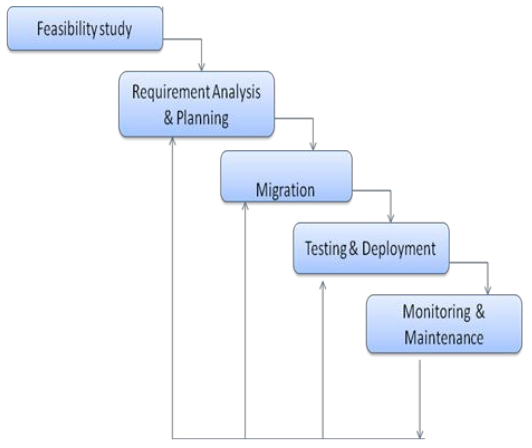
\includegraphics[width=\textwidth]{images/fuenf-phasen-wasserfall-modell.png}
\caption{Das Fünf-Phasen-Wasserfallmodell aus \protect\citeflow{fivephases} }
\label{fuenf-phasen-wasserfall-modell}
\end{center}
\end{figure}
\begin{description}
	\item[Phase 1 - Machbarkeitsstudie] In dieser Phase wird ergebnisoffen 
geprüft, ob die Migration einer Anwendung technisch und wirtschaftlich möglich 
und sinnvoll ist. Dabei wird nicht nur die Anwendung selbst analysiert, sondern 
auch alle Rahmenbedingungen, die Einfluss auf das Verhalten des Systems ausüben 
können. Außerdem wird eine detaillierte Kosten-Nutzen-Analyse erstellt.	

	\item[Phase 2 - Anforderungsanalyse und -Planung] Um die zu migrierende 
Anwendung und ihre Anforderungen zu verstehen, wird in der Planungsphase die 
bestehende IT-Umgebung unter Berücksichtigung der genannten, die Migration 
beeinflussenden Faktoren (siehe  Kapitel 
\ref{cha:migration_bestimmende_faktoren}) 
genau begutachtet. Gilt die Anwendung auch nach Begutachtung als zur Migration 
geeignet, werden der Return on Investment (ROI) sowie die Total Cost of 
Ownership (TCO) berechnet, um die durch die Migration entstehende 
Kostenvorteile 
zu verstehen.
	
	\item[Phase 3 - Migration] Die existierende Anwendung wird in die Cloud 
portiert und in Hinblick auf Leistungsfähigkeit und Performanz strukturiert 
getestet. Zum Schluss wird die neue Plattform in einem User Acceptance Testing 
(UAT) validiert. 
	
	\item[Phase 4 - Tests und Auslieferung] Die Daten aus der Produktion 
werden in die Cloud portiert. Anschließend wird die Software erneut getestet 
und freigegeben. In dieser Phase ist ein hoher Grade an Überwachung und Support 
nötig, um unvorhergesehene Probleme auffangen zu können. Unter Umständen wird 
parallel zum Start der Cloud-Anwendung die Altsoftware zunächst weiter 
betrieben.

	\item[Phase 5 - Überwachung und Wartung] Nach der Migration in die 
Cloud ist es naturgemäß notwendig, die Leistungserfüllung durch den Anbieter in 
Hinblick auf Leistungsfähigkeit, Verfügbarkeit und Sicherheit zu überwachen um 
gegebenenfalls Gegenmaßnahmen einleiten zu können.
\end{description}

\subsection{Migrationsformen}
\citeflow{exploring_the_factors} identifizieren vier Formen, in denen eine 
Migration ablaufen kann.
\begin{description}
	\item[Ersetzen] Einzelne Komponenten einer bestehenden Anwendung werden 
durch Dienste in der Cloud ersetzt. Andere Komponenten, die mit diesen 
ersetzten Komponenten interagieren werden umkonfiguriert.
	\item[Partielle Migration] Anstatt Komponenten durch Cloud-Dienste zu 
ersetzen, werden sie in die Cloud migriert.
	\item[Migration der ganzen Anwendung] Häufig werden Anwendungen in die 
Cloud migriert, indem die virtuellen Maschinen auf denen sie laufen in die 
Cloud umgezogen werden, ohne dass größere Anpassungen nötig wären.
	\item[Cloudify] Die Anwendung wird in Gänze an die Cloud und ihre 
Charakteristika angepasst und mit Cloud Diensten neu entwickelt.
\end{description}

\subsection{Salesforce}

\subsection{Ideen}
\begin{description}
	\item[Migration] Sicht eines Unternehmens, das seine 
On-Promise-Software in die Cloud schiebt versus ISV
\end{description}


\begin{comment}

\subsection{Herausforderungen in Migrationsprojekten als zu berücksichtigende 
Faktoren}
Um die Eignung einer Anwendung für eine Migration in die Cloud zu prüfen, 
schlagen \pcite{}{}{fivephases} die Berücksichtigung der folgenden der 
folgenden wirtschaftlichen und technischen Faktoren vor. Um diese Faktoren in 
einem geordneten Prozess zu berücksichtigen, führen sie ein Vorgehensmodell 
ein. Dieses Vorgehensmodell hat den Vorteil, dass es an bestehende Strukturen 
und Begrifflichkeiten anknüpft und sich deshalb besonders gut vergleichen, 
ergänzen und diskutieren lässt. Aus diesem Grund soll es den Rahmen dieser 
Arbeit bilden.

\subsubsection{Wirtschaftliche Faktoren}

\subsubsection{Technische Faktoren}




\subsubsection{Organisationsform als Einflussfaktor}
\citeflow{fivephases} identifizieren die Organisationsstruktur, beziehungsweise 
deren Größe und Komplexität und insbesondere drei Formen als 
wesentliche Einflussfaktoren für dieses Vorgehensmodell. Zu diesem Ergebnis 
kommen auch \citeflow{Pahl2013}.
\begin{description}
	\item[Große Unternehmen] haben gewachsene, komplexe IT-Strukturen, die 
umso detailliertere Analysen der Cloud-Eignung einzelner Anwendungen 
erforderlich machen und eine Schrittweise Migration nahelegen, bei der 
zunächst einfache Standardanwendungen wie E-Mail-Anwendungen migriert werden. 
Komplexe Anwendungen folgen sobald Erfahrungen im Cloud-Umfeld gesammelt wurden 
und gegebenenfalls fertige Anwendungen in der Cloud bereits existieren.
	\item[Kleinere und mittlere Unternehmen] haben gegenüber großen 
Unternehmen nicht nur den Vorteil einer kleineren, weniger komplexen 
IT-Landschaft. Bestehende Unternehmensprozesse lassen sich auch leichter an die 
Cloud-Nutzung anpassen, sodass sich viele bereits in der Cloud existierende 
Cloud-Anwendungen als SaaS nutzen lassen. Durch die nutzungsabhängige 
Bepreisung lassen sich in der Cloud möglicherweise Anwendungen nutzen, die 
bisher zu teuer oder zu komplex waren. Die nutzungsabhängige Bezahlung birgt 
allerdings wie bereits geschildert auch Risiken, die neben den anderen Faktoren 
ebenfalls vor der Migrationsentscheidung berücksichtigt werden sollten.
	\item[Regierungsorganisationen] dürften regelmäßig zwei Spezifika 
aufweisen, die bei der Prüfung der Cloud-Eignung einer Anwendung zu prüfen 
sind. Erstens sind sie in besonderem Maße, teilweise durch Gesetze, zur 
Kontrolle über die eigenen Daten und Funktionsfähigkeit ihrer Anwendungen 
gezwungen. Zweitens übersteigt die orts-, amts- oder ministerienübergreifende 
Zusammenarbeit die Komplexität von großen Unternehmen bei weitem. 
\end{description}



\subsection{Methoden zur Anforderungsermittlung in Migrationsprojekten}
\subsection{Aktuelle und prognostizierte Ressourcennutzung}
\subsection{Auswahl des Migrationsziels in der Cloud}
\subsection{Kostenabschätzung der Cloud-Lösung}

\newpage
\subsection{Abbildungen}

\begin{figure}[h]
\begin{center}

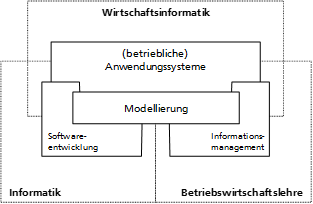
\includegraphics[width=10cm]{images/Abb2_3.png}
\caption{Einordnung der Wirtschaftsinformatik (angelehnt an Fink et al. 2001)}
\label{Abbildung2_3}
\end{center}
\end{figure}
Bitte achten Sie darauf, dass alle vorhandenen Abbildungen und Tabellen in einem inhaltlichen Zusammenhang mit dem Text stehen und Sie auf die entsprechende Abbildung (bspw. Abbildung 1) verweisen.
\subsection{Tabellen}
%hier Tabelle einfügen
\begin{table}[h]
\centering
\begin{tabular}{ccc}
\hline \textbf{Attribute} &\textbf{Typ}  & \textbf{1. Ausprägung (Beispiel)} \\ 
\hline Titel & \textit{STRING}& Aktiengesetz (AktG)  \\ 
Text& \textit{STRING} &  [Text des AktG]\\ 
Gültig von & \textit{DATE} & 01.01.2010 \\ 
Gültig bis & \textit{DATE} & - \\ 
Dok.-Besitzer & \textit{STRING} & Rechtsabteilung \\ 
Quelle & \textit{STRING}  & Deutsche Gesetze \\ 
Verplichtungsgrad & \textit{STRING} & verplichtend \\ 
\hline 
\end{tabular} 
\caption{Attribute der Anforderungsquellen im Metamodell}
\label{tab:tabelle 1}
\end{table}
\par\medskip

Tabelle 1 stellt eine beispielhafte Tabelle dar
\end{comment}